% -*- mode: fundamental -*-

% A tour of the bsc compiler for BSV/BH
% Initial version by Rishiyur S. Nikhil, begun on June 10, 2026

\documentclass[11pt]{article}

% ================================================================
\usepackage[latin1]{inputenc}
\usepackage[T1]{fontenc}
\usepackage{latexsym}
\usepackage{makeidx}
\usepackage{alltt}
\usepackage{verbatim}
\usepackage{fancyvrb}
% \usepackage{moreverb}
\usepackage{index}
\usepackage{ae}
\usepackage{aecompl}

  \usepackage[pdftex,colorlinks=true,bookmarksopen, pdfstartview=FitH,
              linkcolor=blue, citecolor=blue, urlcolor=blue]{hyperref}
  \pdfcompresslevel=9
  \usepackage[pdftex]{graphicx}

\usepackage{xcolor}
\hypersetup{
  colorlinks,
  linkcolor=blue,
}

% Documentation for 'listings': https://www.overleaf.com/learn/latex/Code_listing
\usepackage{listings}

\lstdefinestyle{mystyle}{
    frame=single,
    rulecolor = \color{black},
    commentstyle=\normalfont\color{red},
    basicstyle=\ttfamily\footnotesize,
    breaklines=true,
    keepspaces=false,
    showspaces=false,
    showtabs=false,
    escapeinside={@}{@}
}

\lstset{style=mystyle}

%    backgroundcolor=\color{lightgray},
%    keywordstyle=\color{magenta},
%    numberstyle=\tiny\color{gray},
%    stringstyle=\color{purple},
%    breakatwhitespace=false,
%    showstringspaces=false,
%    tabsize=2,
%    captionpos=b,
%    numbers=left,
%    numbersep=5pt,

% \lstset{
%   columns=fullflexible,
%   basicstyle=\ttfamily,
%   rulecolor = \color{black},
%   commentstyle=\mycommentstyle,
%   escapechar=\$,
%   showstringspaces = false,
% }
% \newcommand{\mycommentstyle}{\normalfont\itshape}

% ================================================================
% Table of contents packages etc.

% For additional short table of contents:
%     https://www.ctan.org/tex-archive/macros/latex/contrib/shorttoc/
\usepackage[tight]{shorttoc}

% For changing spacing between entries in toc
\usepackage{tocloft}

% ================================================================

% HORIZONTAL MARGINS
% Left margin, odd pages: 1.25 inch (0.25 + 1)
\setlength{\oddsidemargin}{0.25in}
% Left margin, even pages: 1.25 inch (0 + 1)
\setlength{\evensidemargin}{0.25in}
% Text width 6 inch (so other margin is 1.25 inch).
\setlength{\textwidth}{6in}
% ----------------
% VERTICAL MARGINS
% Top margin 0.5 inch (-0.5 + 1)
\setlength{\topmargin}{-0.5in}
% Head height 0.25 inch (where page headers go)
\setlength{\headheight}{0.25in}
% Head separation 0.25 inch (between header and top line of text)
\setlength{\headsep}{0.25in}
% Text height 9 inch (so bottom margin 1 in)
\setlength{\textheight}{9in}
% ----------------
% PARAGRAPH INDENTATION
\setlength{\parindent}{0in}
% SPACE BETWEEN PARAGRAPHS
\setlength{\parskip}{\medskipamount}
% ----------------
% STRUTS
% HORIZONTAL STRUT.  One argument (width).
\newcommand{\hstrut}[1]{\hspace*{#1}}
% VERTICAL STRUT. Two arguments (offset from baseline, height).
\newcommand{\vstrut}[2]{\rule[#1]{0in}{#2}}
% ----------------
% HORIZONTAL LINE ACROSS PAGE:
\newcommand{\hdivider}{\noindent\mbox{}\hrulefill\mbox{}} 
% ----------------
% EMPTY BOXES OF VARIOUS WIDTHS, FOR INDENTATION
\newcommand{\hm}{\hspace*{1em}}
\newcommand{\hmm}{\hspace*{2em}}
\newcommand{\hmmm}{\hspace*{3em}}
\newcommand{\hmmmm}{\hspace*{4em}}
% ----------------
% VARIOUS CONVENIENT WIDTHS RELATIVE TO THE TEXT WIDTH, FOR BOXES.
\newlength{\hlessmm}
\setlength{\hlessmm}{\textwidth}
\addtolength{\hlessmm}{-2em}

\newlength{\hlessmmmm}
\setlength{\hlessmmmm}{\textwidth}
\addtolength{\hlessmmmm}{-4em}
% ----------------
% ``TIGHTLIST'' ENVIRONMENT (no para space betwee items, small indent)
\newenvironment{tightlist}%
{\begin{list}{$\bullet$}{%
    \setlength{\topsep}{0in}
    \setlength{\partopsep}{0in}
    \setlength{\itemsep}{0in}
    \setlength{\parsep}{0in}
    \setlength{\leftmargin}{1.5em}
    \setlength{\rightmargin}{0in}
    \setlength{\itemindent}{0in}
}
}%
{\end{list}
}
% ----------------
% ITALICISE WORDS
\newcommand{\ie}{\emph{i.e.,}}
\newcommand{\eg}{\emph{e.g.,}}
\newcommand{\Eg}{\emph{E.g.,}}
\newcommand{\etc}{\emph{etc.}}
\newcommand{\via}{\emph{via}}
\newcommand{\vs}{\emph{vs.}}
% ----------------
% Require numbering for subsubsections, and show them in table of contents
\setcounter{secnumdepth}{3}
\setcounter{tocdepth}{3}
% ----------------
\graphicspath{ {Figures/} }
% ----------------
% CODE FONT (e.g. {\cf x := 0}).
\newcommand{\cf}{\footnotesize\tt}
\newcommand{\T}[1]{{\footnotesize\tt #1}}
\newcommand{\N}[1]{{\normalfont #1}}
% ----------------
% The bsc compiler and BSV language
\newcommand{\BSC}{{\it{}bsc}}
\newcommand{\BSCREPOLINK}{\url{https://github.com/B-Lang-org/bsc}}
\newcommand{\BSV}{\bf{BSV}}
\newcommand{\BH}{\bf{BH}}
\newcommand{\BSVBH}{\bf{BSV/BH}}
\newcommand{\BLUESIM}{\bf{Bluesim}}
\newcommand{\VERILATOR}{\bf{Verilator}}
\newcommand{\GHC}{\bf{ghc}}
% ----------------
% RISC-V Simulators etc.
\newcommand{\SPIKE}{\bf{Spike}}
\newcommand{\SAIL}{\bf{Sail}}
\newcommand{\CISSR}{\bf{Cissr}}
\newcommand{\TESTRIG}{\bf{TestRIG}}
\newcommand{\QUICKCHECK}{\bf{QuickCheck}}
% ----------------
% KEYWORDS
\newcommand{\kw}[1]{{\bf #1}}
% ----------------
% Inputting verbatim code fragments
\newcommand{\SHOWCODE}[1]{{\footnotesize\input{#1}}}

% ----------------------------------------------------------------
% ----------------------------------------------------------------
% HERE BEGINS THE DOCUMENT

\newcommand{\copyrightnotice}{\copyright 2026 B-Lang.org}

% ================================================================

\begin{document}

% ================================================================
% Title etc.

\begin{center}
{\Large\bf A Developers' Guide for the {\BSC} compiler}

{\Large\bf Authors: Various \footnotesize{(see end of \S\ref{sec:overview})}}

{\bf Version: June 11, 2026}

\vspace*{5ex}

{\bf Abstract}

\begin{minipage}{0.8\textwidth}

This document is intended to assist people who are studying or
modifying the Haskell source code of the {\BSC} compiler, including
developers (maintainers/bug-fixers/improvers) and PR-reviewers.

\vspace*{1ex}

It may also be useful for others who wish to instrument {\BSC} for
analysis and/or connection to other tools ({\eg} formal verification
tools, LSP servers, code browsers, ...).

\vspace*{1ex}

We assume the reader has a basic knowledge of Haskell (nothing
advanced). \S\ref{sec:Haskell} is a brief cheat sheet.

\end{minipage}

\end{center}

% ****************************************************************
% Table of contents

\hdivider

\label{sec:longtoc}

\tableofcontents

% ****************************************************************
% Short table of contents
%
% {\small \shorttoc{Short Table of Contents}{1} }
%

\hdivider

% ****************************************************************

\section{Overview}

\label{sec:overview}

The {\BSC} compiler is invoked like any Unix executable from the shell
command-line with command-line flags and arguments.  The {\tt bsc}
command actually invokes a small script that ultimately invokes the
main compiler binary. ``\mbox{\tt bsc -help}'' will list the
command-line flags and arguments.

The {\BSC} compiler is written in Haskell, and is compiled to a binary
using the {\GHC} Glasgow Haskell Compiler.

The entry point of any Haskell program is the function {\tt main}
(\S\ref{sec:main}).

The main compiler flow is in the {\tt compilePackage} Haskell
function.  It is structured as a sequence of \emph{stages} (or
compiler passes), described in more detail later in
\S\ref{sec:compilePackage} and illustrated in
Figure~\ref{fig:compilePackage}.

Each stage transforms a data structure input to a data structure
output, and these are passed sequentially from stage to stage.  The
data structures are an internal representation of the {\BSVBH}
program, plus auxiliary information.

As indicated in the figure, the intermediate data structures are of
three major types:
\begin{tabbing}
\hm \= CSyntax \hm \= \kill
    \> CSyntax \hm \> Concrete Syntax, augmented with type information ($\ddagger$\ref{sec:CSyntax}) \\
    \> ISyntax \hm \> Intermediate representation ($\ddagger$\ref{sec:ISyntax}) \\
    \> ASyntax \hm \> Abstract Transition Syntax ($\ddagger$\ref{sec:ASyntax})
\end{tabbing}

\vspace{5ex}

{\bf Authors of this document} This is an open-source document and is
expected to be updated by various people to keep it in sync with the
{\BSC} compiler as {\BSC} evolves over time.  The git log should list
the contributors and their contributions to this document.  This
document was begun by Rishiyur S. Nikhil on 2026-06-10, as part of his
own journey to learn the internals of {\BSC} (to that date he was not
an author any of the {\BSC} compiler source code).

% ****************************************************************

\section{Resources}

The {\BSC} compiler is in this repository (repo): \\
\hmmm \url{https://github.com/B-Lang-org/bsc}
The compiler is written in fairly vanilla Haskell and exists in a
collection of Haskell source code files ({\tt .hs} and {\tt .lhs}
extensions).  The compiler, per se, is mostly in the {\tt src/comp/}
directory; the {\BSV} and {\BH} parsers are in {\tt src/comp/Parser/}.

In the repo, the file {\tt INSTALL.md} describes how to build (compile
and link) the {\BSC} compiler.  {\BSC} is built using the {\GHC}
Haskell compiler.  This document also has some notes on building, in
\S\ref{sec:build}.

NOTE: \hfill \fbox{
\begin{minipage}{0.9\textwidth}

  Most \emph{users} of {\BSC} do not need to build {\BSC} from
  scratch.  Pre-built binaries are available for many Linux platforms
  and for MacOS; please see the ``Download ... Releases'' link in the
  repo's README.

\end{minipage}}


% ****************************************************************

\section{Notation in this document}

Each listing display in the sections that follow is a gloss of a
Haskell function in the source code, {\ie} a summary, omitting much
detail.  These are intended as a high-level ``road map'' for the
actual code, are best read side-by-side with the actual code.

Our focus in these listings is on the ``flow'' of major functions, and
so we omit the actual ``plumbing'' that connects inputs and outputs of
functions. Haskell being a pure functional language, all plumbing is
with explicit inputs and outputs (no side-effects on external data
structures).  Function inputs are arguments ``\mbox{\tt f x}'', and
functions outputs are typically bound with ``\mbox{\tt let y = f x}''
let-bindings, or ``\mbox{\tt y <- f x}'' monadic bindings, or directly
returned into a surrounding expression.  The details of plumbing
values between functions are best seen in the actual source code.

Many listings begin with the name of the file containing the code.
\begin{lstlisting}[language=Haskell]
@\it\color{red}File:@ bsc/src/comp/bsc.hs
\end{lstlisting}

Haskell identifiers are shown as is, ``\verb|x|'', if the Haskell
file/module context is obvious, or prefixed with its Haskell module
name to clarify, ``\verb|module_name::x|''.

NOTE: \hfill \fbox{\begin{minipage}{0.9\textwidth} A possible point of
confusion: What Haskell calls a {\tt module} (a large-program
organizing construct) is called a {\tt package} in {\BSVBH} because in
{\BSVBH} the word ``module'' is reserved for hardware items.
\end{minipage}}

Function call chains are shown indented like this ({\tt f1} calls {\tt
f2} which calls {\tt f3} which calls ...):
\begin{lstlisting}[language=Haskell]
    f1
      f2
        f3
          ...
\end{lstlisting}

Functions called in sequence (in a monadic \verb|do|) are listed
vertically in sequence, like this:

\begin{lstlisting}[language=Haskell]
    f1
    f2
    ...
\end{lstlisting}

Functions called as alternatives (in if-then-elses/cases) are listed
vertically in sequence with vertical bars, like this:

\begin{lstlisting}[language=Haskell]
    | f1
    | f2
    | ...
\end{lstlisting}

A list of items is shown using the usual Haskell square-bracket list notation: [item]

% ****************************************************************

\section{Top-level of the {\BSC} compiler}

The entry point for the {\BSC} compiler program, like any Haskell
program, is the function {\tt main} (\S\ref{sec:main}).

% ================================================================

\subsection{{\tt Main\_bsc::main}, {\tt Main\_bsc::hmain} and {\tt Main\_bsc::hmain'}}

\label{sec:main}

{\tt main} just invokes {\tt hmain} within a wrapper that catches any
exceptions raised therein.

{\tt hmain} performs one of several top-level actions depending on
command-line flags; one of those alternatives is to invoke {\tt main'}
for compiling a {\BSVBH} program.

\begin{lstlisting}[language=Haskell]
@\it\color{red}File:@ bsc/src/comp/bsc.hs

main            -- Haskell top-level function
  hmain           -- Top-level of @\BSC@, via @\tt bsCatch@
  | help            -- print flags help and exit
  | helpHidden      -- print flags, hidden flags, and exit
  | usage           -- print usage and exit
  | main'           -- process a source file
  | vLink ()        -- verilog link
  | simLink ()      -- bluesim link
\end{lstlisting}

\verb|hmain'|, when invoked with -u, follows the import chain and
locates all files/packages to be recompiled and calls
\verb|compilePackage| on each such file.

\begin{lstlisting}[language=Haskell]
@\it\color{red}File:@ bsc/src/comp/bsc.hs

main'
  compile_with_deps    -- when invoked with -u
    chkDeps              -- uses @\tt{}Depend::parseFile@
                         -- and returns [pkg] needing recompilation
    compilePackage     -- on each file in [pkg]

| compile_no_deps      -- when invoked without -u
    Depend::parseFile    -- which returns pkg
    compilePackage       -- on the specified file
\end{lstlisting}

See \S\ref{sec:Parsing} for: \verb|Depend::parseFile|.

% ================================================================

\subsection{Compiling a package (file) \hmm {\tt Main\_bsc::compilePackage}}

\label{sec:compilePackage}

{\tt compilePackage} embodies the top-level ``flow'' of the compiler
and is a sequential composition of many stages, or passes.  These are
shown in Figure~\ref{fig:compilePackage}.
\begin{figure}[htbp]
  \centerline{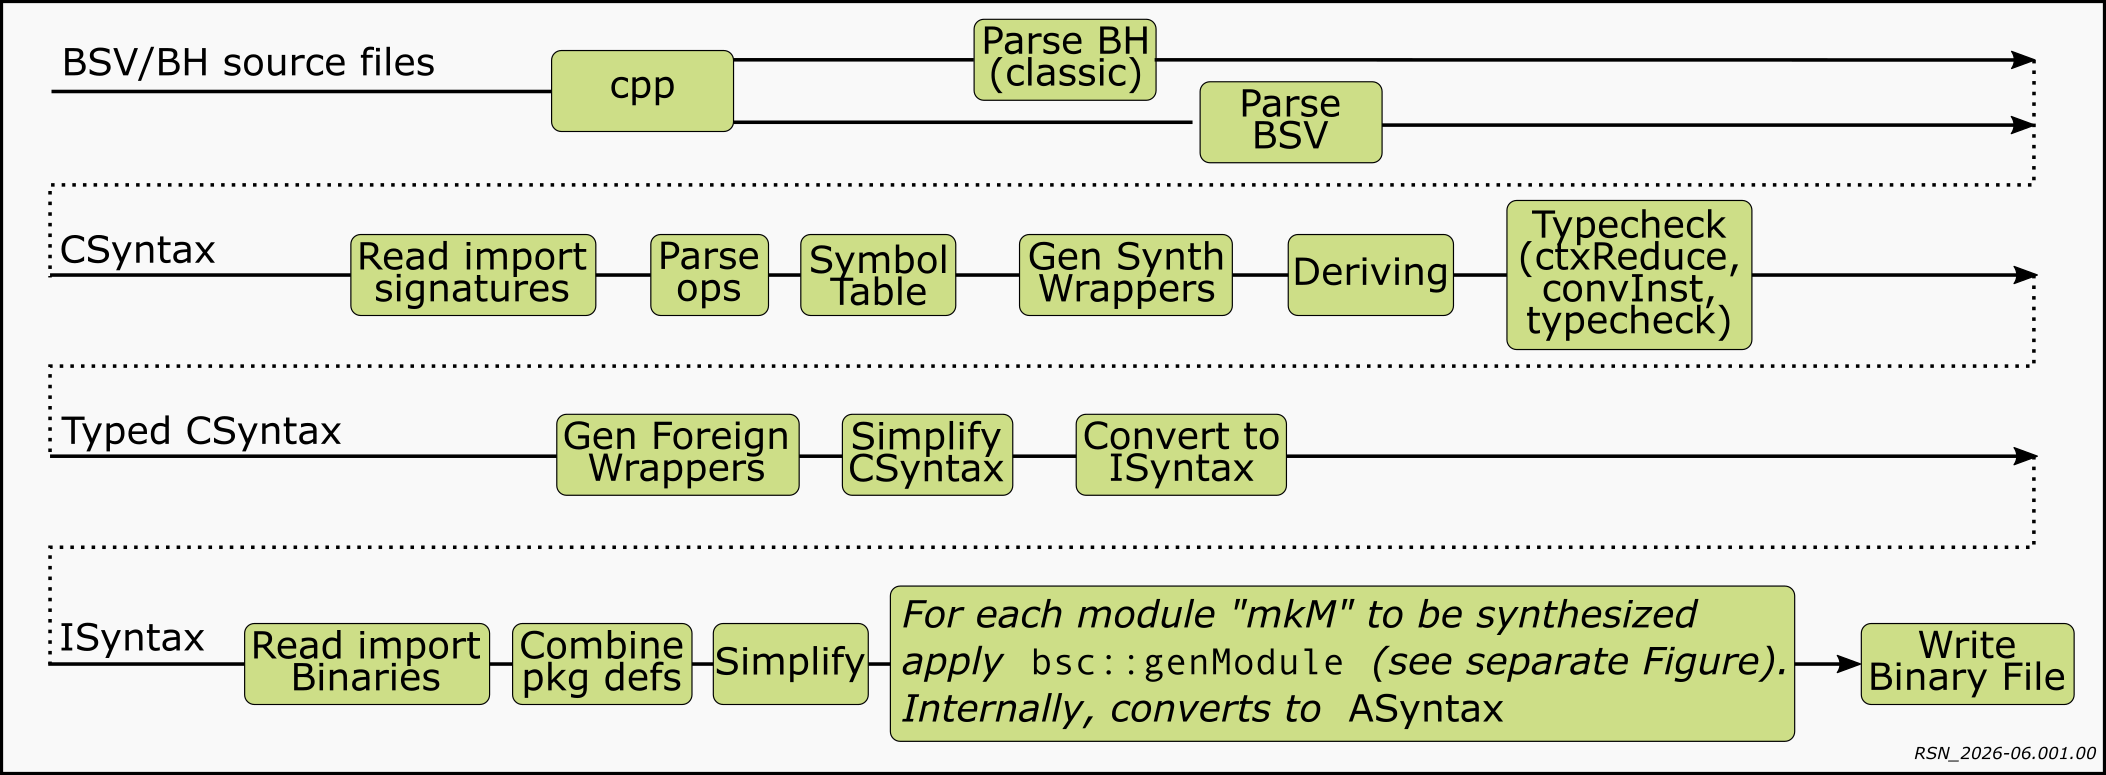
\includegraphics[width=\textwidth]{Figures/RSN_2026-06.001.00_bsc_stages.png}}
  \caption{\label{fig:compilePackage}
           Major stages in flow of {\BSC} compiler (see function {\tt compilePacakage})}
\end{figure}

Towards the end, a stage invokes {\tt genModule} to actually produce
Verilog or Bluesim output.  Internally, it converts ISyntax into
ASyntax. {\tt genModule} is discussed in more detail in
\S\ref{sec:genModule}.

Each of the stages is surrounded by \verb|start|, \verb|stats| and
\verb|dump| calls.  They are meant for providing info to the user on
statistics and current state of internal representation.  We omit
those calls in the gloss below.

\begin{lstlisting}[language=Haskell]
@\it\color{red}File:@ bsc/src/comp/bsc.hs

compilePackage
-- The incoming BSV/BH package is the final arg
-- We are working with CSyntax (incoming package)
    readImports    -- read signatures of imported packages
    parseOps       -- in pkg ParseOp.  Handles infix ops
                   --     (@$\ddagger$\ref{sec:parseOps}@)
    mkSymTab       -- Generate a global symbol table
                   --     (MakeSymTab:: @$\ddagger$\ref{sec:mkSymTab}@)
                   --     First of several times that the table is built
    genFuncWrap    -- Turn `noinline' into module definitions
    genWrap        -- Generate wrapper for Verilog interface.
    mkSymTab       -- because added new types (MakeSymTab:: @$\ddagger$\ref{sec:mkSymTab}@)
                   --      and typeclass instances for those types
    addFuncWrap    -- Re-add function definitions for `noinline'
    derive         -- Turn deriving into instance declarations
    mkSymTab       -- because Deriving added new instances
                   --     (MakeSymTab:: @$\ddagger$\ref{sec:mkSymTab}@)
    cCtxReduceIO   -- Reduce the contexts as far as possible
    mkSymTab       -- because possibly changed types of top-level definitions
                   -- (MakeSymTab:: @$\ddagger$\ref{sec:mkSymTab}@)
    cConvInst      -- Turn instance declarations into ordinary definitions
    cTypeCheck     -- Type check and insert dictionaries
                   --     (TypeCheck:: @$\ddagger$\ref{sec:cTypeCheck}@)
-- We are now working with: Typed CSyntax

    genForeign     -- Generate wrapper info for foreign function imports
                   --     (always happens, even when not generating for modules)
    mkGenFileHeader,
    genDPIWrappers -- Generate VPI wrappers for foreign function imports
    simplify       -- Simplify a little

    iConvPackage   -- Convert to internal abstract syntax
    iPCheck        -- @\bf TODO: What does this do?@
-- We are now working with ISyntax

    map Data.Map.lookup
                   -- Read binary interface files
                   --   (just looks up in data structure, not read files?) 
    map adjEnv     -- adjust the "raw" packages and then add back their
                   --   signatures so they can be put into the current
                   --   IPackage for linking info.
		   --   Injects the "magic" variables genC and genVerilog
    mkSymTab       -- For "genModule" we construct a symbol table that
                   --     includes all defs, not just user visible defs
		   --     (MakeSymTab:: @$\ddagger$\ref{sec:mkSymTab}@)
    fixupDefs      -- @\bf TODO: What does this do?@
    iSimplify      -- @\bf TODO: What does this do?@
    iPCheck        -- @\bf TODO: What does this do?@

    orderGens      -- @\bf TODO: What does this do?@

    gen            -- Generate code for all requested modules (recursive)
      genModule      -- Synthesize a module
      compileCDefToIDef
                     -- @\bf TODO: What does this do?@
    genUserSign    -- Generate the user-visible type signature
    genEverythingSign
                   -- Generate a type signature where everything is visible
    genBinFile     -- Generate binary version of the internal tree .bo file
\end{lstlisting}

% ================================================================

\subsection{Creating (and re-creating) the symbol table {\tt MakeSymTab::mkSymTab}}

\label{sec:mkSymTab}

{\tt mkSymTab} is invoked in {\tt compilePackage}
(\S\ref{sec:compilePackage}). It is invoked multiple times,
presumably to keep it in sync with latest transformations to the
program representation.

\begin{lstlisting}[language=Haskell]
@\it\color{red}File:@ bsc/src/comp/MakeSymTab.hs

mkSymTab :: ErrorHandle -> CPackage -> IO SymTab
\end{lstlisting}

The symbol table is actually 6 tables: constructor names, type names, ...

% ================================================================

\subsection{Handling infix/prefix ops and associativities \hmm {\tt ParseOp::parseOps}}

\label{sec:parseOps}

{\tt parseOps} handles the various infix, prefix and distfix operators
with varying precedences and associativities.

\begin{lstlisting}[language=Haskell]
@\it\color{red}File:@ bsc/src/comp/ParseOp.hs

parseOps :: ErrorHandle -> CPackage -> IO CPackage
\end{lstlisting}

% ================================================================

\subsection{Annotating module input/output ports \hmm {\tt GenWrap::genWrap}}

\label{sec:genWrap}

\begin{lstlisting}[language=Haskell]
@\it\color{red}File:@ bsc/src/comp/GenWrap.hs

-- creates wrappers for separately compiled modules: wraps pack/unpack around method
-- arguments and results; surfaces method ready signals
-- Pragma are module specific
genWrap :: ErrorHandle -> Flags -> [String] -> Bool -> CPackage -> SymTab ->
           IO (CPackage, [WrapInfo])
\end{lstlisting}

{\tt genWrap} looks at all modules being synthesized, and for each
interface, creates primitive interfaces (bit vectors, prim actions,
...).

It's done before type-checking, but with symbol table info.  Question:
why is this wrapper generated so early?

This is only the first part.  The full wrapper happens after
compilation, including scheduling etc.

% ****************************************************************

\section{Major internal representations of the program}

% ================================================================

\subsection{Concrete Syntax \hmm {\tt CSyntax}}

\label{sec:CSyntax}

CSyntax presumably stands for ``Concrete Syntax''.  This is the
``parse tree'' representation produced by the {\BSVBH} parsers, and is
used for the first several stages of the compiler.

% ================================================================

\subsection{Intermediate Syntax \hmm {\tt ISyntax}}

\label{sec:ISyntax}

ISyntax presumably stands for ``Intermediate Syntax''. and is used in
the middle stages of the compiler.  This is the representation that is
put out into ``{\tt .bo}'' intermediate files.

ISyntax is much smaller than CSyntax. It is a ``SystemF-ish''
representation ({\ie}, includes type application).

There is a pre- and post-elaboration distinction of ISyntax \\
\hmm Pre: packages
\hmm Post: modules

% ================================================================

\subsection{Abstract Transition Syntax \hmm {\tt ASyntax}}

\label{sec:ASyntax}

ASyntax presumably stands for ``Abstract Transition Syntax'' (from
James Hoe's thesis), and is used in the final stages of the compiler
dealing with rules, scheduling, and for producing the Bluesim and
Verilog outputs.

% ****************************************************************

\section{Parsing \hmm {\tt Depend::parseFile}}

\label{sec:Parsing}

\verb|parseFile| is invoked in {\tt compilePackage} (\S\ref{sec:compilePackage}).

\vspace*{1ex}

\begin{lstlisting}[language=Haskell]
@\it\color{red}File:@ bsc/src/comp/Depend.hs

parseFile     -- run CPP, dump CPP output, parse, check name,
              --   dump CSyntax, stats
              --   returns a CPackage
  parseSrc      -- wrapper to detect file encoding errors
    parseSrc'     -- Parse a BH or BSV file
\end{lstlisting}

The {\BSVBH} split happens in \verb|parseSrc'|, depending on the filename extension: ``{\tt .bsv}'' for {\BSV} or ``{\tt .bs}'' for {\BH}.

\begin{lstlisting}[language=Haskell]
@\it\color{red}File:@ bsc/src/comp/Depend.hs

parseSrc'
| Parser.Classic::pPackage    -- BH parse
| Parser.BSV::bsvParseString  -- BSV parse
\end{lstlisting}

Historical note: \hfill\fbox{
\begin{minipage}{0.8\textwidth}

  Originally (ca. 2000), the language was just called {\bf Bluespec},
  and there was only one syntax, hence the file extension ``{\tt
  .bs}''.  It had/has Haskell-like syntax, and today we call it
  ``Bluespec Classic'' or {\BH}.

  \vspace{1ex}

  Later (ca. 2004) we added the {\BSV} syntax (SystemVerilog-like) as
  an alternative.

\end{minipage}}

The only difference between {\BSV} and {\BH} is the syntax and these
two front-end parsers. Both of them produce a CSyntax output, after
which there is no difference in the rest of the compiler; in
particular {\BSV} and {\BH} share the same semantics.  Using {\BSV} or
{\BH} is just a personal preference.  A single design can mix packages
written in {\BSV} with packages written in {\BH}

% ================================================================

\subsection{Parsing {\BH} \hmm {\tt CParser::pPackage}}

\label{sec:parsing_BH}

The {\BH} parser top-level:

\begin{lstlisting}[language=Haskell]
@\it\color{red}File:@ bsc/src/comp/Parser/Classic/CParser.hs

pPackage  -- Parse into CSyntax
\end{lstlisting}

% ================================================================

\subsection{Parsing {\BSV} \hmm {\tt CVParser::bsvParseString}}

\label{sec:parsing_BSV}

The {\BSV} parser top-level:

\begin{lstlisting}[language=Haskell]
@\it\color{red}File:@ bsc/src/comp/Parser/BSV/CVParser.lhs

bsvParseString  -- Parse, then desugar, into CSyntax
\end{lstlisting}

After parsing there are ``desugaring'' steps which:

\begin{itemize}

  \item convert from imperative syntax into pure functional form.  For
    example, {\BSV} syntax allows a variable to be ``updated'' in an
    Action-block, and these are converted into pure functional form.

  \item for-loops are converted into recursive functions.

  \item {\tt StmtFSM} constructs are converted into algebraic types [TODO: confirm?]

\end{itemize}

This results in some redundant info for the parser, like {\tt Action}
and {\tt action} keywords [TODO: clarify].

% ****************************************************************

\section{Type checking \hmm {\tt TypeCheck::cTypeCheck}}

\label{sec:cTypeCheck}

\begin{lstlisting}[language=Haskell]
@\it\color{red}File:@ bsc/src/comp/ParseOp.hs

cTypeCheck :: ErrorHandle -> Flags -> SymTab -> CPackage -> IO (CPackage, Bool, S.Set Id)
\end{lstlisting}

{\tt cTypecheck} converts between different variants of CSyntax.
There are different invariants at different stages.

% ****************************************************************

\section{Code generation \hmm {\tt Main\_bsc::genModule}}

\label{sec:genModule}

\verb|genModule| synthesizes a module (generates Verilog or Bluesim
code).  It, in turn, consists of a number of stages, shown in
Figure~\ref{fig:genModule_flow}.
\begin{figure}[htbp]
  \centerline{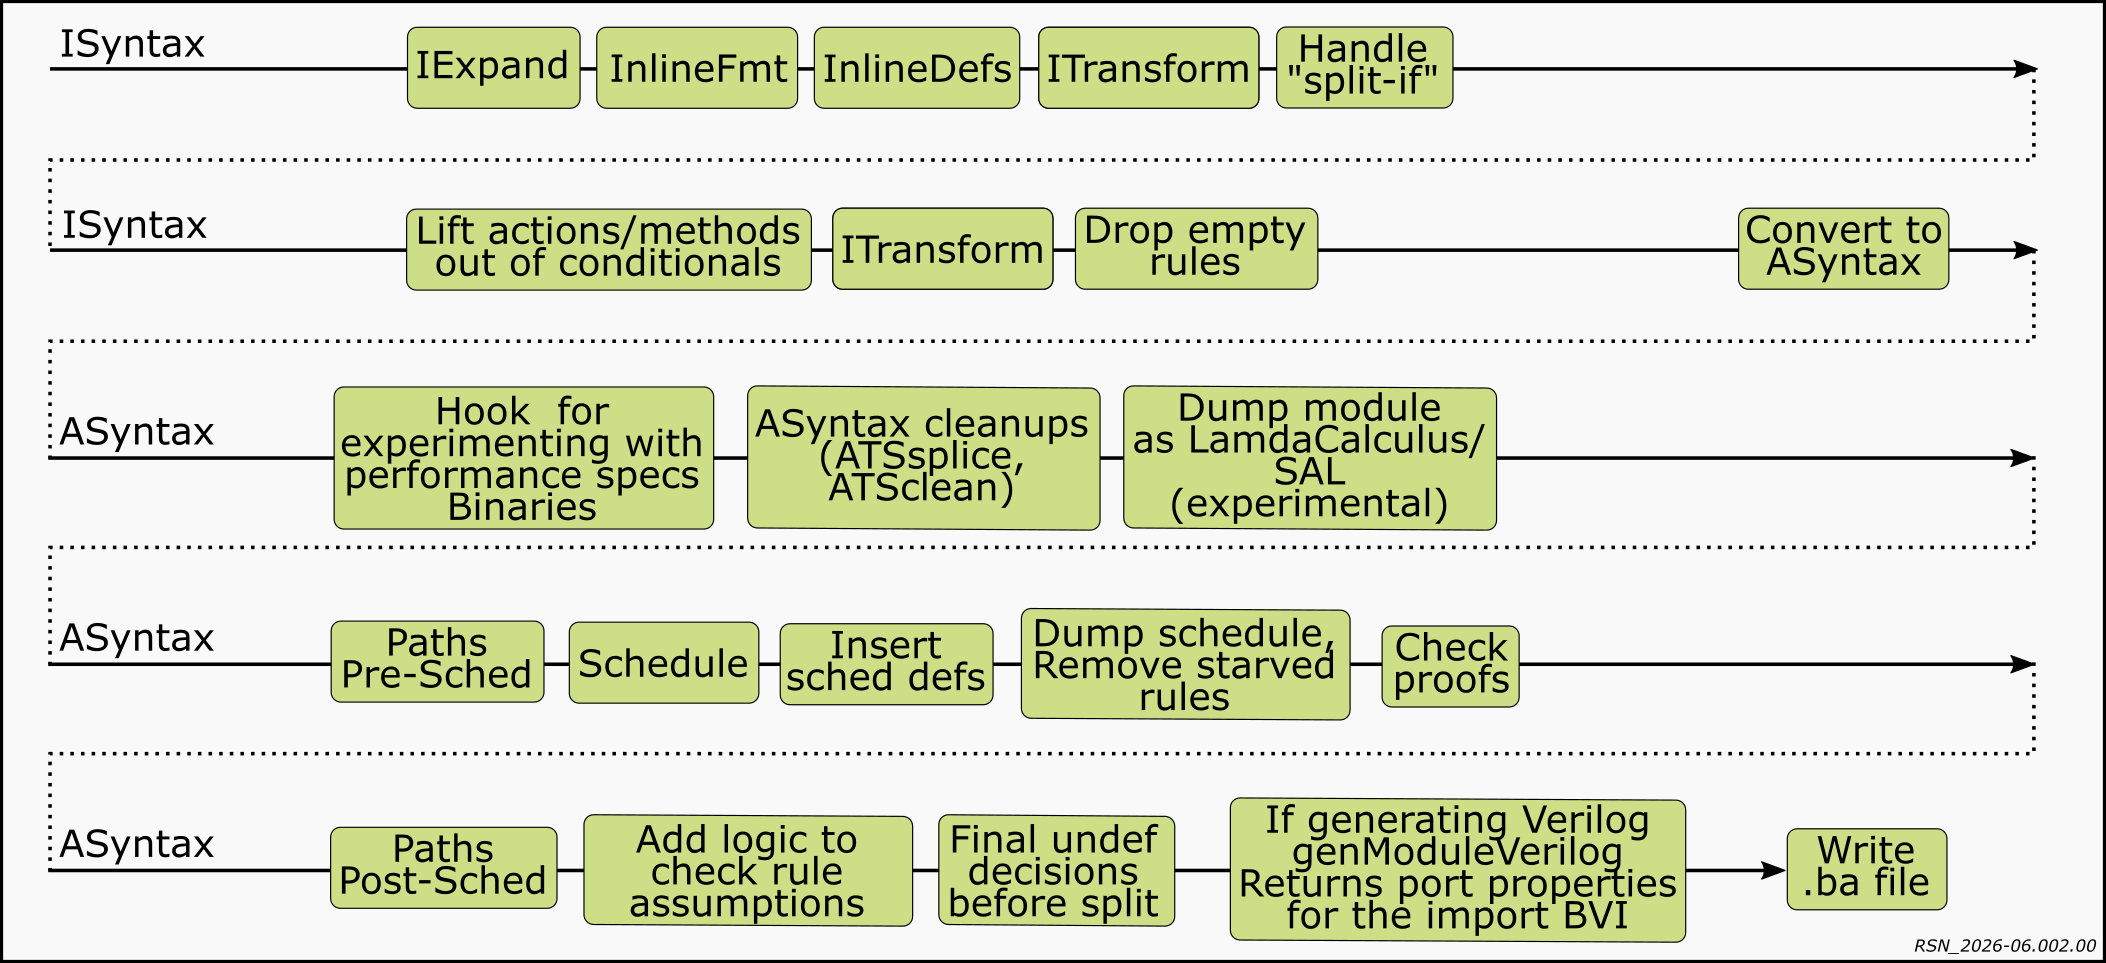
\includegraphics[width=\textwidth]{Figures/RSN_2026-06.002.00_bsc_genModule.png}}
  \caption{\label{fig:genModule_flow}
           Major stages in flow of function {\tt genModule})}
\end{figure}
Internally, it converts ISyntax into ASyntax.

\begin{lstlisting}[language=Haskell]
@\it\color{red}File:@ bsc/src/comp/bsc.hs

genModule
-- Input is in ISyntax
    iExpand        -- "run" the module monad
    iNormTypes     -- normalize types (handle lingering SizeOf)
    iInlineFmt
    iInline        -- Inline defs
    iTransform
    iSplitIf       -- Split rules containing if statements
    iLift          -- Lift actions/methods out of conds,
                   --   and merge where possible
    iTransform     -- Transform to simpler form (take 2)
    iParams        -- Inline expressions for submodule instantiation
                   --  parameters, or separate them into localparam defs
		   --  instead of wire defs
    iDropRules     -- Drop empty rules
    aConv          -- Generate ATS ("Abstract Transition Syntax",
                   --   cf. James Hoe thesis)

-- We are now working with ASyntax (type @\tt APackage@ file @\tt ASyntax.hs@)

    flattenInstTree
    aRankMethCalls -- append ranks to method names and calls for
                   --   "performance guarantees"
    aTaskSplice    -- splice in identifiers set by ActionValue tasks
                   --   into ATaskAction calls
    aCleanup       -- clean up ATS (merge any ME calls to same action
                   --   in same rule)

    convAPackageToLambdaCalc; dump
                   -- experimental dump to lambda calc (for formal verif)
    convAPackageToSAL; dump
                   -- experimental dump to SAL (for formal verif)

    aPathsPreSched -- Build path graph for everything except rules
    aSchedule      -- Schedule
    aAddScheduleDefs
                   -- Add CAN_FIRE and WILL_FIRE defs based on the schedule
    aDumpSchedule
    aCheckProofs   -- prove any proof obligations accumulated at this point
                   --   the obligations are removed from the module
    aPathsPostSched
                   -- Add scheduler edges to the path graph
                   --   (assume pathGraphInfo is consistent with
		   --    amod_checked, because at most only a few rules
		   --    have been removed since amod_clean)
    aNoInline      -- lift all no-inline func calls
                   --   and assign instance names to them
    aAddCFConditionWires,
                   -- add scheduling assumptions (ME, CF, etc.) to APackage
      aAddSchedAssumps
                   --   (in two steps)
    aRemoveAssumps -- move assumption actions into rule bodies
    aDropUndet     -- drop ASAny with "chosen" values
                   -- just before the split because other paths add new expressions
                   -- and because we might choose more undets in pathsPostSched

-- The amod doesn't change beyond this point

    apkg_external_wires
                   -- save wireinfo
    getAPackageFieldInfos

    genModuleVerilog
                   -- if generating Verilog
    writeABin      -- if genABin

    deffun         -- "wrappergen" handling value methods with
                   -- constant True output (@\bf TODO@: always ready?)
\end{lstlisting}

% ****************************************************************

\section{Notes on building the {\BSC} compiler (compiling and linking)}

\label{sec:build}.

NOTE: \hfill \fbox{
\begin{minipage}{0.9\textwidth}

  Most \emph{users} of {\BSC} do not need to build {\BSC} from
  scratch.  Pre-built binaries are available for many Linux platforms
  and for MacOS; please see the ``Download ... Releases'' link in the
  repo's README.

\end{minipage}}

{\BSC} is built using the {\GHC} Haskell compiler.  The file {\tt
INSTALL.md} in the repo {\BSCREPOLINK} is the definitive document on
how to do this.  This section has some additional notes about the
process.

\emph{To be written ...}

% ****************************************************************
% ****************************************************************
% ****************************************************************

\appendix

% ****************************************************************

\section{Brief Haskell cheat sheet}

\label{sec:Haskell}

We describe here the basic Haskell notations used in the {\BSC} source
code.  This is not intended to be a Haskell tutorial; many such
tutorials exist on the web.  However, descriptions here may be enough
to enable reading the source code.

\emph{This section needs to be written ... but the headings below
indicate the relevant Haskell features one should know in order to
read the source code.}

{\bf {\tt .hs} and {\tt .lhs} (``literate Haskell'') files}

{\bf Indentation and ``off-side rule''}

{\bf Top-level function type declarations and definitions}

{\bf Function application, partial application}

{\bf IO monad}

{\bf {\tt do} notation, {\tt <-} binding, {\tt return}}

{\bf {\tt let} bindings}

{\bf \$ composition (right-associative)}

{\bf List notation, list comprehensions}

{\bf Lambda expresions}

{\bf if-then-else and case expressions}

{\bf Haskell modules, imports and exports}

NOTE: \hfill \fbox{\begin{minipage}{0.9\textwidth}

  A possible point of confusion: What Haskell calls a {\tt module} (a
  large-program organizing construct) is called a {\tt package} in
  {\BSVBH} because in {\BSVBH} the word ``module'' is reserved for
  hardware items.

  \vspace*{1ex}

  A Haskell {\tt module} or {\BSVBH} {\tt package} allows a large
  program to be split into smaller pieces (usually each in its own
  file), with controlled visibility of identifiers across the boundary
  (using imports and exports, and qualified-names). It is purely a
  source-code organizing mechanimsm, and has no hardware significance.

\end{minipage}}

{\bf Algebraic type definitions, {\tt deriving}, {\tt show}}

{\bf Typeclasses and instances}

The {\BSC} code itself does not seem to define any new Haskell
typeclasses, just instances of existing typeclasses.

% ****************************************************************

\end{document}
